\documentclass[12pt,a4paper]{article}

% ------------------ Pakiety ------------------

\usepackage{multicol}
%\usepackage[polish]{babel}
%\usepackage[T1]{fontenc}
%\usepackage[utf8]{inputenc}
%\usepackage[T1]{fontenc}
%\usepackage{polski}
%\usepackage{lmodern}
\usepackage{graphicx}
\usepackage{hyperref}
\usepackage{fontspec}            % for XeLaTeX / LuaLaTeX
\defaultfontfeatures{Ligatures=TeX}
\setmainfont{Latin Modern Roman}
\usepackage[polish]{babel}       % babel supports polish with LuaLaTeX
\usepackage{lmodern}             % optional for PDFLaTeX fallback
\graphicspath{{resources/}}      % look for images in lab03/resources/
\usepackage{setspace}
\usepackage{titlesec}
\usepackage{array}
\usepackage[utf8]{inputenc}
\usepackage{polski}
\usepackage{lmodern}
\usepackage{float}


% ------------------ Ustawienia ------------------

\geometry{margin=2.5cm}
\setstretch{1.3}
\titleformat{\section}{\large\bfseries}{\thesection.}{1em}{}
\titleformat{\subsection}{\normalsize\bfseries}{\thesubsection.}{1em}{}
\hypersetup{
    colorlinks=true,
    linkcolor=black,
    urlcolor=blue,
    pdftitle={Planowanie procesu wdrożenia produktu informatycznego za pomocą UML}
}

% ------------------ Dane ------------------

\title{Uniwersytet Gdański
Wydział Matematyki, Fizyki i Informatyki
Instytut Informatyki}
\author{Oliver Gruba, Maciej Nasiadka}

\begin{document}
\maketitle
\begin{table}
    \centering
    \begin{tabular}{|>{\raggedright\arraybackslash}p{0.5\linewidth}|>{\raggedright\arraybackslash}p{0.4\linewidth}|}\hline
         Imię i Nazwisko& Oliver Gruba \\
         & Maciej Nasiadka\\\hline
         Nazwa uczelni& Uniwersytet Gdański\\\hline
         Kierunek& Informatyka (profil praktyczny)\\\hline
         Prowadzący& dr inż. Stanisław Witkowski\\\hline
         Specjalność& —\\\hline
         Nazwa ćwiczenia& Planowanie procesu wdrożenia produktu informatycznego za pomocą
UML\\\hline
         Numer sprawozdania& 1\\\hline
         Data zajęć& 16.10.2025\\\hline
         Data oddania& 22.10.2025\\\hline
         Miejscę na ocenę& \\ \hline
    \end{tabular}
\end{table}

\clearpage

% ------------------ Dokument ------------------

\tableofcontents
\newpage

\section{Wprowadzenie}

Celem niniejszego sprawozdania jest przedstawienie procesu planowania wdrożenia produktu informatycznego z wykorzystaniem języka UML (Unified Modeling Language). UML jest uniwersalnym i standaryzowanym językiem modelowania, który umożliwia graficzne odwzorowanie zarówno struktury, jak i zachowania systemu informatycznego. Dzięki swojej elastyczności może być stosowany w różnych fazach cyklu życia oprogramowania: od analizy wymagań, poprzez projektowanie, aż po implementację i testowanie.

W procesie projektowania systemów informatycznych UML odgrywa kluczową rolę w komunikacji między analitykami, projektantami, programistami oraz interesariuszami projektu. Poprzez czytelną reprezentację wizualną umożliwia on łatwiejsze zrozumienie koncepcji systemu, identyfikację potencjalnych błędów projektowych na wczesnym etapie oraz zapewnienie spójności między dokumentacją a implementacją.

Zastosowanie UML pozwala również na tworzenie modeli niezależnych od konkretnych technologii implementacyjnych, co czyni go użytecznym narzędziem w różnorodnych środowiskach projektowych, zarówno w podejściach tradycyjnych (kaskadowych), jak i zwinnych (agile).

\section{Elementy języka UML}

Język UML składa się z zestawu notacji i reguł, które umożliwiają opisanie zarówno statycznych, jak i dynamicznych aspektów systemu. Każdy typ diagramu ma określony cel i zakres zastosowania, co pozwala na wielowymiarową analizę projektowanego rozwiązania.

\subsection{Diagramy strukturalne}

Diagramy strukturalne przedstawiają statyczną organizację systemu, czyli sposób, w jaki jego elementy są ze sobą powiązane niezależnie od dynamiki działania. Opisują one architekturę systemu, strukturę danych oraz relacje pomiędzy obiektami.

Najczęściej stosowane diagramy strukturalne to:
\begin{itemize}
\item Diagram klas - prezentuje strukturę obiektową systemu poprzez klasy, ich atrybuty, operacje oraz relacje między nimi. Ułatwia zrozumienie hierarchii dziedziczenia i zależności między komponentami logicznymi.
\item Diagram komponentów - obrazuje logiczną strukturę modułów systemu oraz ich interfejsy, co umożliwia planowanie integracji i zależności między elementami oprogramowania.
\item Diagram wdrożenia - ukazuje fizyczne rozmieszczenie komponentów w środowisku uruchomieniowym, w tym serwery, urządzenia klienckie i bazy danych.
\item Diagram pakietów - grupuje powiązane elementy modelu w logiczne jednostki, co poprawia przejrzystość dużych projektów i umożliwia modularne podejście do projektowania.
\end{itemize}

\subsection{Diagramy behawioralne}

Diagramy behawioralne służą do opisu dynamicznych aspektów systemu, czyli sposobu, w jaki reaguje on na działania użytkowników, zdarzenia zewnętrzne lub wewnętrzne zmiany stanu. Dzięki nim można modelować logikę procesów biznesowych oraz przepływy danych.

Najczęściej wykorzystywane diagramy behawioralne to:
\begin{itemize}
\item Diagram przypadków użycia - prezentuje funkcjonalność systemu z punktu widzenia użytkownika, wskazując, jakie działania może on wykonywać i jakie cele może osiągnąć.
\item Diagram czynności - odwzorowuje przepływ czynności, decyzji i równoległych procesów, co czyni go przydatnym w analizie przepływów pracy (workflow).
\item Diagram sekwencji - przedstawia wymianę komunikatów pomiędzy obiektami w czasie, pozwalając zrozumieć kolejność interakcji i zależności przy realizacji przypadków użycia.
\end{itemize}

\subsection{Elementy graficzne}

UML wykorzystuje zestaw standaryzowanych symboli graficznych \ref{fig:UML_diagram_example}, które ułatwiają komunikację między projektantami. Przykładowe elementy to: prostokąty (reprezentujące klasy lub komponenty), owale (przypadki użycia), romby (decyzje), strzałki (relacje lub przepływy komunikatów) oraz piktogramy ludzików (aktorzy).
Dzięki spójności i jednoznaczności notacji możliwe jest efektywne odczytywanie modeli nawet przez osoby z różnych zespołów projektowych.

\begin{figure}[ht]
\centering
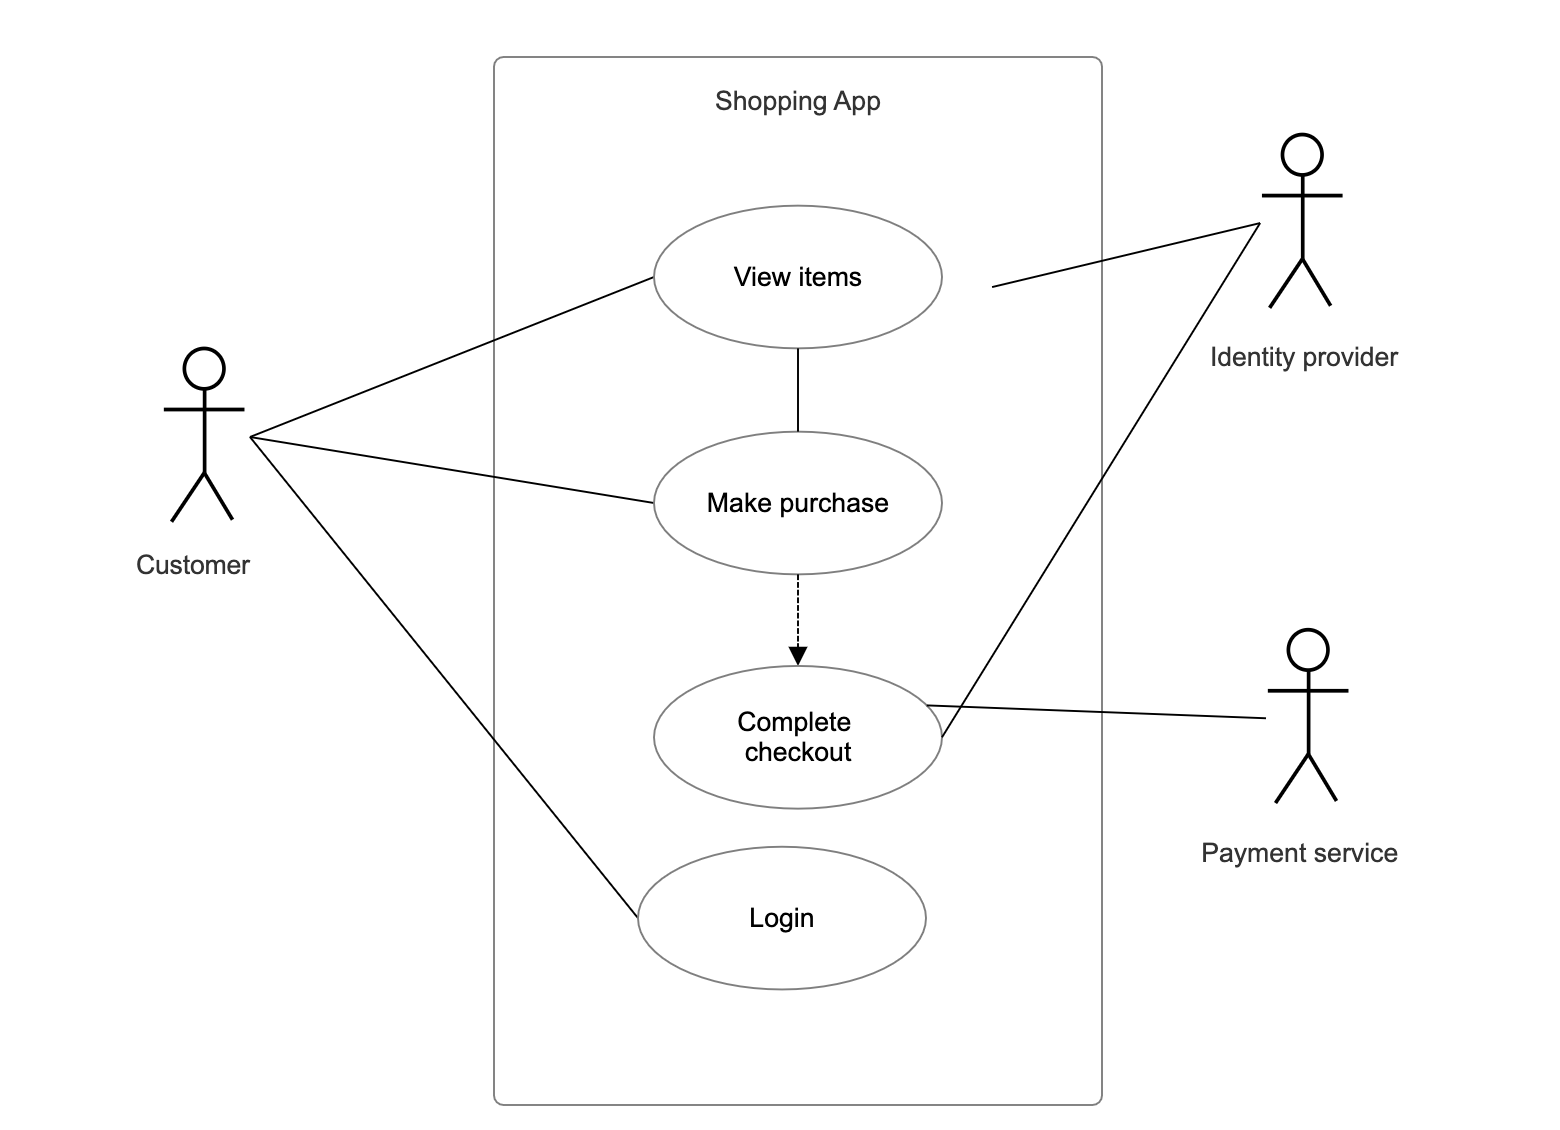
\includegraphics[width=0.5\linewidth]{UML_diagram_example.png}
\caption{Przykład wyglądu diagramu UML przedstawiający przykład elementów graficznych (przypadków użycia i aktorów)}
\label{fig:UML_diagram_example}
\end{figure}

\section{Modelowanie wymagań za pomocą przypadków użycia}

Modelowanie wymagań w UML koncentruje się na identyfikacji interakcji między użytkownikami systemu a jego funkcjami. Diagram przypadków użycia (use case diagram) stanowi podstawę dokumentacji analitycznej i jest często pierwszym krokiem w procesie modelowania systemu. \ref{fig:system_diagram_example}

\begin{figure}[H]
\centering
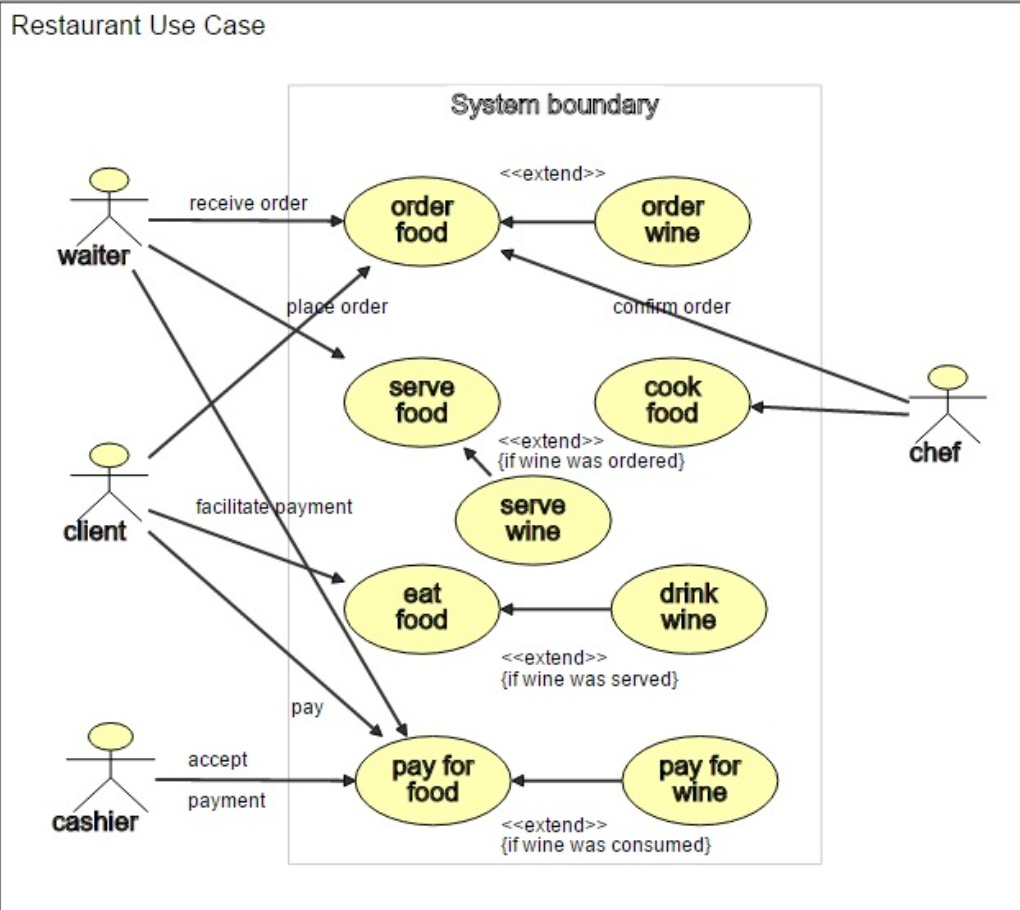
\includegraphics[width=0.5\linewidth]{system_diagram_example.png}
\caption{(Przykład modelu przypadku użycia dla restauracji)}
\label{fig:system_diagram_example}
\end{figure}

Każdy przypadek użycia reprezentuje pojedynczy scenariusz interakcji użytkownika (aktora) z systemem, prowadzący do osiągnięcia konkretnego celu. Dzięki temu możliwe jest:
\begin{itemize}
\item zidentyfikowanie wszystkich typów użytkowników (aktorów) i ich ról,
\item określenie zakresu odpowiedzialności systemu oraz granic jego funkcjonalności,
\item doprecyzowanie wymagań funkcjonalnych i niefunkcjonalnych.
\end{itemize}

Taki model jest szczególnie pomocny w komunikacji z klientem i interesariuszami, ponieważ opisuje zachowanie systemu w sposób zrozumiały bez konieczności znajomości technicznych aspektów projektu. W dalszej fazie projektowania przypadki użycia mogą stanowić punkt wyjścia do tworzenia diagramów sekwencji lub czynności, które opisują szczegółową logikę realizacji poszczególnych funkcji.

\section{Diagramy czynności i sekwencji}
\subsection{Diagram czynności}

Diagram czynności (activity diagram) pozwala na modelowanie przepływu procesów w systemie. Może być używany zarówno do przedstawienia logiki działania pojedynczego przypadku użycia, jak i całych procesów biznesowych. Dzięki możliwości reprezentacji rozgałęzień, decyzji oraz równoległego wykonywania czynności, diagram ten stanowi efektywne narzędzie do analizy algorytmów i procesów roboczych.

\subsection{Diagram sekwencji}

Diagram sekwencji (sequence diagram) koncentruje się na interakcjach pomiędzy obiektami w czasie. Umożliwia analizę komunikacji w ramach realizacji danego przypadku użycia, identyfikację zależności między komponentami oraz potencjalnych problemów z synchronizacją czy nadmiernym sprzężeniem elementów.
Poprawnie opracowany diagram sekwencji jest nieocenionym źródłem informacji podczas implementacji, ponieważ precyzyjnie odwzorowuje logikę przepływu danych i komunikatów.

\section{Modelowanie klas i powiązań między nimi}

Model klas jest centralnym elementem projektowania obiektowego, stanowiąc logiczną strukturę całego systemu. Klasy reprezentują byty rzeczywiste lub abstrakcyjne, które posiadają atrybuty (dane) oraz metody (operacje).

Rodzaje powiązań między klasami obejmują:
\begin{itemize}
\item Dziedziczenie - umożliwia tworzenie hierarchii klas poprzez przenoszenie wspólnych cech do klasy bazowej.
\item Asocjację - określa logiczne powiązania między klasami, np. relację klient-zamówienie.
\item Agregację - relacja „całość-część”, w której elementy mogą istnieć niezależnie od całości.
\item Kompozycję - silniejsze powiązanie, w którym elementy nie mogą istnieć bez obiektu nadrzędnego (np. pokój jest częścią domu).
\end{itemize}

Model klas jest podstawą do generowania kodu źródłowego w językach obiektowych takich jak Java, C\# czy Python, a jego poprawna konstrukcja wpływa na jakość, skalowalność i łatwość utrzymania systemu.

\section{Diagram komponentów}

Diagram komponentów obrazuje logiczną strukturę systemu w kontekście współpracy między jego modułami. Komponent może reprezentować fragment aplikacji, bibliotekę, usługę sieciową, mikrousługę lub interfejs API.
Tego rodzaju diagram pomaga w planowaniu architektury systemu, identyfikacji zależności między modułami oraz analizie potencjalnych miejsc integracji z zewnętrznymi systemami. Jest szczególnie przydatny przy projektach rozproszonych lub opartych na architekturze mikroserwisowej.

\section{Podział modelu na pakiety}

Podział modelu na pakiety (package diagram) pozwala na hierarchiczne uporządkowanie elementów modelu UML. Dzięki temu możliwe jest efektywne zarządzanie dużymi projektami, utrzymanie przejrzystości i podział pracy między zespoły.

Zalety stosowania pakietów:
\begin{itemize}
\item łatwiejsze zarządzanie złożonością modelu,
\item możliwość ponownego wykorzystania komponentów i klas w innych projektach,
\item równoległe opracowywanie różnych części systemu przez niezależne zespoły projektowe.
\end{itemize}

\section{Modelowanie wdrożenia systemu}

Model wdrożenia (deployment diagram) przedstawia fizyczną architekturę systemu, w tym sposób rozmieszczenia jego komponentów na węzłach sprzętowych.
Diagram ten określa relacje pomiędzy serwerami, stacjami roboczymi, bazami danych, aplikacjami klienckimi oraz oprogramowaniem pośrednim (middleware).
W kontekście planowania wdrożenia produktu informatycznego, taki model pozwala:
\begin{itemize}
\item zaplanować wymagania dotyczące infrastruktury sprzętowej i sieciowej,
\item określić sposób dystrybucji i aktualizacji komponentów systemu,
\item zaplanować procesy monitorowania, bezpieczeństwa i utrzymania po wdrożeniu.
\end{itemize}

Dzięki temu modelowanie wdrożenia wspiera planowanie realistycznej, stabilnej i skalowalnej architektury systemu informatycznego.

\section{Dostępne narzędzia do projektowania UML i dobre praktyki}

\subsection{Przegląd narzędzi komercyjnych}
Na rynku istnieje wiele zaawansowanych narzędzi komercyjnych wspierających modelowanie UML:

\begin{itemize}
    \item Visual Paradigm - rozbudowane środowisko z funkcjami analizy i generowania kodu. Oferuje pełne wsparcie dla wszystkich typów diagramów UML 2.x, automatyczne generowanie dokumentacji oraz zaawansowaną integrację z popularnymi środowiskami programistycznymi (Eclipse, IntelliJ IDEA, Visual Studio). Wyróżnia się intuicyjnym interfejsem oraz możliwością transformacji modeli w kod w wielu językach programowania (Java, C++, C\#, PHP).
    
    \item Enterprise Architect (Sparx Systems) - kompleksowe narzędzie do zarządzania projektami IT. Poza standardowym UML oferuje wsparcie dla BPMN, SysML oraz wielu innych notacji modelowania. Wyróżnia się możliwościami symulacji modeli, zarządzania wymaganiami oraz generowania raportów. Szczególnie przydatne w dużych przedsiębiorstwach z rozbudowaną infrastrukturą IT oraz w projektach wymagających zgodności z rygorystycznymi standardami.
    
    \item IBM Rational Software Architect - zaawansowane środowisko projektowe integrujące się z ekosystemem IBM. Zapewnia kompleksowe wsparcie dla cyklu wytwarzania oprogramowania, od modelowania architektury po generowanie kodu i testy. Zawiera rozbudowane mechanizmy transformacji modeli oraz walidacji architektonicznej.
    
    \item MagicDraw - narzędzie cenione za intuicyjny interfejs i wydajność przy pracy z dużymi modelami. Oferuje zaawansowane mechanizmy współpracy zespołowej, kontroli wersji oraz integracji z narzędziami ALM (Application Lifecycle Management). Szczególnie popularne w branżach wymagających wysokiej niezawodności, jak lotnictwo czy obronność.
\end{itemize}

\subsection{Rozwiązania open-source i darmowe}
Alternatywą dla rozwiązań komercyjnych są narzędzia open-source i freeware:

\begin{itemize}
    \item StarUML - lekka aplikacja z otwartą architekturą wtyczek. Obsługuje standard UML 2.x i oferuje podstawowe funkcje generowania kodu. Interfejs przypomina klasyczny Microsoft Visio, co ułatwia adaptację nowym użytkownikom. Dostępna jest wersja darmowa z ograniczoną funkcjonalnością oraz płatna wersja Pro z rozszerzonymi możliwościami.
    
    \item Umbrello UML Modeller - darmowe narzędzie dostępne głównie dla systemów Linux/KDE, oferujące wsparcie dla większości typów diagramów UML. Umożliwia import kodu źródłowego (C++, Java, Python) i generowanie dokumentacji. Wyróżnia się niskimi wymaganiami sprzętowymi i prostotą obsługi.
    
    \item ArgoUML - jedno z najstarszych otwartych narzędzi UML, nadal rozwijane przez społeczność. Oferuje wsparcie dla głównych typów diagramów UML 1.4, automatyczną walidację modelu oraz generowanie kodu w kilku językach programowania. Interfejs może wydawać się przestarzały, ale narzędzie jest stabilne i sprawdzone w wielu projektach.
    
    \item Modelio - zaawansowana platforma modelowania z otwartym kodem źródłowym. Wspiera UML 2.5, BPMN oraz SysML. Oferuje modułową architekturę umożliwiającą rozszerzanie funkcjonalności poprzez wtyczki. Dostępne są darmowa wersja podstawowa oraz płatne rozszerzenia dla zastosowań profesjonalnych.
\end{itemize}

\subsection{Narzędzia online i oparte na chmurze}
Coraz większą popularność zyskują rozwiązania dostępne przez przeglądarkę:

\begin{itemize}
    \item Lucidchart - intuicyjne narzędzie online umożliwiające tworzenie różnych typów diagramów, w tym UML. Wyróżnia się możliwościami współpracy w czasie rzeczywistym, bogatą biblioteką szablonów oraz integracją z popularnymi narzędziami (G Suite, Microsoft Office, Slack). Oferuje model freemium z ograniczoną wersją darmową.
    
    \item Draw.io (Diagrams.net) - darmowe narzędzie do tworzenia diagramów online z możliwością lokalnej instalacji. Choć nie jest dedykowane wyłącznie dla UML, oferuje przyzwoite wsparcie dla większości typów diagramów. Zapewnia integrację z popularnymi usługami przechowywania danych (Google Drive, OneDrive, Dropbox).
    
    \item GenMyModel - specjalistyczne narzędzie online do modelowania UML z zaawansowanymi funkcjami walidacji i generowania kodu. Zaprojektowane z myślą o pracy zespołowej i kontroli wersji. Oferuje zarówno darmowy plan podstawowy, jak i płatne subskrypcje z rozszerzonymi funkcjami.
    
    \item Visual Paradigm Online - webowa wersja popularnego narzędzia desktop. Zapewnia dostęp do kluczowych funkcji modelowania UML z dowolnego urządzenia z przeglądarką. Oferuje funkcje współpracy w czasie rzeczywistym oraz integrację z rozwiązaniami chmurowymi.
    
    \item Creately - platforma do współpracy wizualnej z silnym wsparciem dla UML. Wyróżnia się intuicyjnym interfejsem oraz funkcjami umożliwiającymi jednoczesną pracę wielu użytkowników. Oferuje zarówno wersję online, jak i desktop.
\end{itemize}

\subsection{Wtyczki do IDE i rozszerzenia}
Dla programistów preferujących pozostanie w środowisku programistycznym:

\begin{itemize}
    \item PlantUML - rozszerzenie umożliwiające tworzenie diagramów UML za pomocą prostego języka tekstowego. Dostępne jako wtyczka do wielu IDE (VSCode, IntelliJ, Eclipse) oraz narzędzi do dokumentacji. Szczególnie cenione przez zwolenników podejścia "everything as code".
    
    \item UML Designer for Eclipse - rozszerzenie dodające zaawansowane funkcje modelowania UML do Eclipse. Bazuje na Sirius i Eclipse Modeling Framework, oferując pełne wsparcie dla UML 2.5.
    
    \item ObjectAid UML Explorer - lekka wtyczka do Eclipse umożliwiająca wizualizację kodu Java jako diagramów klas UML. Pozwala na automatyczne generowanie diagramów z istniejącego kodu, co jest szczególnie przydatne przy analizie i refaktoryzacji.
    
    \item Mermaid - biblioteka JavaScript umożliwiająca generowanie diagramów z tekstu, podobnie do PlantUML. Zintegrowana z wieloma narzędziami, w tym GitHub, GitLab i VS Code. \ref{fig:mermaid_diagram_example}
\end{itemize}

\begin{figure}[H]
    \centering
    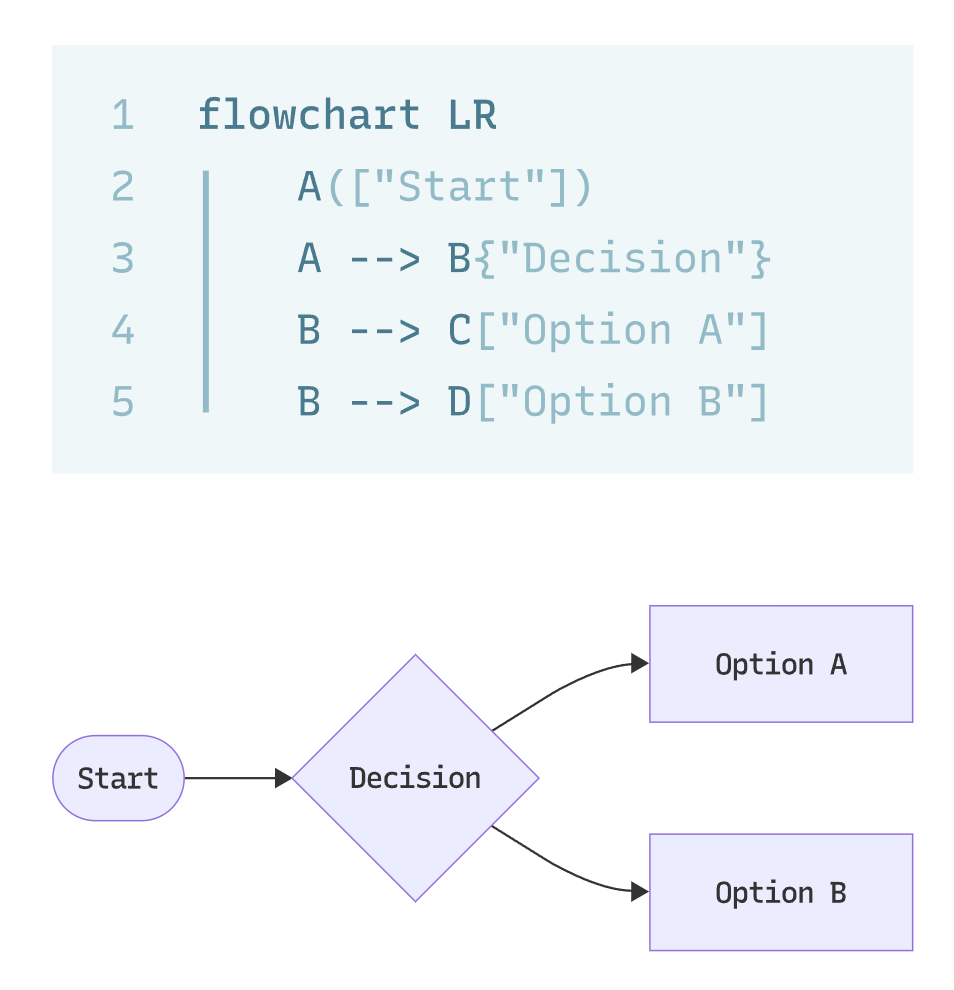
\includegraphics[width=0.5\linewidth]{mermaid_diagram_example.png}
    \caption{Przykład diagramu typu mermaid - kod i postać blokowa}
    \label{fig:mermaid_diagram_example}
\end{figure}

\subsection{Kryteria wyboru narzędzi UML}
Przy wyborze odpowiedniego narzędzia warto uwzględnić następujące kryteria:

\begin{itemize}
    \item Skala projektu - dla małych projektów wystarczające mogą być narzędzia online lub darmowe, podczas gdy duże przedsięwzięcia korporacyjne wymagają zaawansowanych funkcji narzędzi komercyjnych.
    
    \item Zespół i współpraca - istotne są funkcje umożliwiające jednoczesną pracę wielu osób, kontrolę wersji oraz zarządzanie uprawnieniami.
    
    \item Integracja z procesem wytwórczym - kompatybilność z używanymi narzędziami (IDE, systemy kontroli wersji, narzędzia CI/CD) może znacząco wpłynąć na efektywność.
    
    \item Generowanie kodu i inżynieria wsteczna - dla zespołów stosujących podejście model-driven development kluczowa jest jakość generowanego kodu oraz możliwość synchronizacji modelu z istniejącym kodem.
    
    \item Eksport i dokumentacja - możliwość eksportu diagramów do różnych formatów oraz automatycznego generowania dokumentacji.
    
    \item Koszt i licencjonowanie - należy rozważyć nie tylko cenę zakupu, ale również koszty utrzymania, aktualizacji i szkoleń.
\end{itemize}

\subsection{Dobre praktyki w modelowaniu UML}
Efektywne wykorzystanie UML wymaga stosowania sprawdzonych praktyk:

\subsubsection{Praktyki organizacyjne}
\begin{itemize}
    \item Regularność aktualizacji - model UML powinien ewoluować wraz z projektem; regularna aktualizacja modeli zapewnia ich aktualność i użyteczność.
    
    \item Integracja z procesem wytwórczym - modele UML powinny być traktowane jako pełnoprawne artefakty procesu wytwórczego, podlegające takim samym zasadom jak kod źródłowy (przeglądy, kontrola wersji).
    
    \item Dokumentowanie zmian - każda istotna zmiana w modelu powinna być udokumentowana i powiązana z odpowiednimi wymaganiami lub zgłoszeniami.
    
    \item Przechowywanie w repozytorium - modele UML powinny być przechowywane w systemie kontroli wersji, najlepiej w formacie umożliwiającym śledzenie zmian (tekstowy lub XML).
    
    \item Sesje modelowania zespołowego - organizowanie wspólnych sesji modelowania zwiększa zrozumienie systemu i zapewnia spójność wizji wśród członków zespołu.
\end{itemize}

\subsubsection{Praktyki techniczne}
\begin{itemize}
    \item Konwencje nazewnictwa - stosowanie spójnych, jednoznacznych i opisowych nazw dla elementów modelu. Warto ustalić i dokumentować konwencje na początku projektu.
    
    \item Poziom szczegółowości - dopasowanie poziomu szczegółowości modelu do jego celu. Zbyt szczegółowe modele są trudne w utrzymaniu, zbyt ogólne mogą być niewystarczające.
    
    \item Modularyzacja - podział złożonych modeli na mniejsze, zarządzalne moduły za pomocą pakietów i widoków.
    
    \item Konsystencja - zapewnienie spójności między różnymi typami diagramów (np. klasy występujące na diagramie sekwencji powinny być zdefiniowane na diagramie klas).
    
    \item Walidacja - regularne sprawdzanie poprawności modelu pod względem zgodności z metodyką UML oraz wewnętrznej spójności.
    
    \item Komentarze i dokumentacja - dodawanie adnotacji i komentarzy wyjaśniających złożone elementy modelu lub decyzje projektowe.
\end{itemize}

\subsubsection{Praktyki komunikacyjne}
\begin{itemize}
    \item Dostosowanie do odbiorcy - różne diagramy mogą być używane do komunikacji z różnymi interesariuszami (np. diagram przypadków użycia dla klienta, diagram klas dla programistów).
    
    \item Czytelność wizualna - dbanie o przejrzystość diagramów poprzez odpowiednie rozmieszczenie elementów, grupowanie powiązanych obiektów i unikanie nadmiaru informacji na pojedynczym diagramie.
    
    \item Stosowanie widoków - tworzenie dedykowanych widoków modelu podkreślających konkretne aspekty systemu, dostosowanych do potrzeb różnych interesariuszy.
    
    \item Standaryzacja oznaczeń - wykorzystywanie standardowych oznaczeń UML zamiast tworzenia własnych, co ułatwia zrozumienie modelu przez nowe osoby.
\end{itemize}

\subsubsection{Najczęstsze błędy i jak ich unikać}
\begin{itemize}
    \item Nadmierny formalizm - skupianie się na dokładnym przestrzeganiu składni UML kosztem praktycznej użyteczności. Lepiej tworzyć modele, które efektywnie komunikują zamysł, nawet jeśli czasem odchodzą od formalnego standardu.
    
    \item Zbyt szczegółowe modelowanie - próba uwzględnienia wszystkich detali implementacyjnych w modelu. UML powinien koncentrować się na architekturze i kluczowych aspektach, pozostawiając szczegóły implementacyjne kodowi.
    
    \item "Modelowanie dla modelowania" - tworzenie diagramów bez jasnego celu. Każdy diagram powinien odpowiadać na konkretne pytanie lub wspierać konkretny aspekt procesu wytwórczego.
    
    \item Zaniedbanie aktualizacji - nieaktualizowanie modeli wraz z ewolucją systemu, co prowadzi do rozbieżności między dokumentacją a rzeczywistością.
\end{itemize}

\subsection{UML w metodykach zwinnych}
Choć UML kojarzy się często z tradycyjnymi metodami wytwarzania oprogramowania, może być również efektywnie stosowany w projektach zwinnych:

\begin{itemize}
    \item Lekkie modelowanie - tworzenie tylko niezbędnych diagramów, skupiających się na kluczowych elementach systemu.
    
    \item Modelowanie ewolucyjne - rozwijanie modeli równolegle z kodem, stopniowo zwiększając ich szczegółowość.
    
    \item Modelowanie jako komunikacja - używanie UML podczas spotkań zespołu do wyjaśniania koncepcji i planowania implementacji.
    
    \item Diagram jako prototyp - wykorzystywanie diagramów UML do szybkiego prototypowania rozwiązań przed rozpoczęciem implementacji.
    
    \item Integracja z historiami użytkownika - łączenie diagramów przypadków użycia z historiami użytkownika w celu lepszego zrozumienia wymagań.
\end{itemize}

\section{Diagramy UML stworzone w Draw.io}

W celu zilustrowania wcześniej opisanych koncepcji przygotowano zestaw diagramów UML przy użyciu narzędzia Draw.io. Każdy z diagramów przedstawia inny aspekt projektowanego systemu i wspiera dokumentację procesu wdrożenia.

\subsection{Diagram przypadków użycia}
Diagram przypadków użycia prezentuje kluczowych aktorów systemu oraz funkcjonalności, z których korzystają. Dzięki niemu można łatwo zidentyfikować zakres odpowiedzialności systemu oraz powiązania między użytkownikami a usługami informatycznymi. \ref{fig:drawio_use_case}

\begin{figure}[ht]
    \centering
    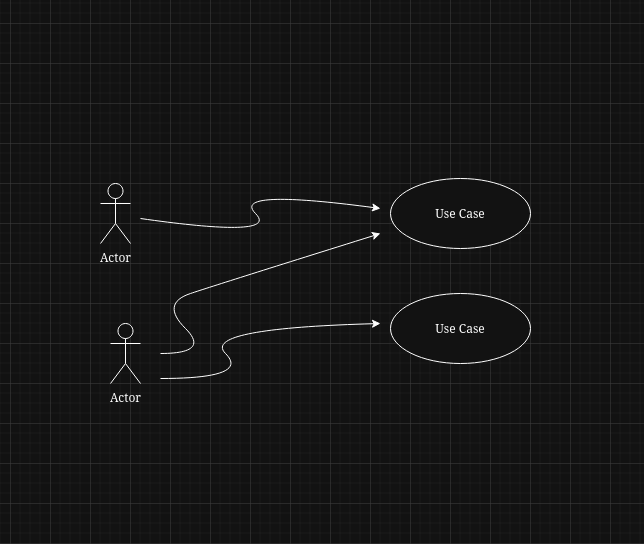
\includegraphics[width=0.75\linewidth]{drawio_use_case.png}
    \caption{Diagram przypadków użycia przygotowany w Draw.io}
    \label{fig:drawio_use_case}
\end{figure}

\subsection{Diagram czynności}
Diagram czynności obrazuje przepływ pracy, decyzje oraz możliwe równoległe ścieżki realizacji procesu. Ułatwia analizę kluczowych kroków wdrożenia i identyfikację potencjalnych miejsc optymalizacji.

\subsection{Diagram wdrożenia}
Diagram wdrożenia prezentuje docelową architekturę środowiska uruchomieniowego wraz z rozlokowaniem komponentów. Pomaga zaplanować konfigurację sprzętową i sieciową oraz określić zależności między elementami infrastruktury. \ref{fig:drawio_deployment}

\begin{figure}[h]
    \centering
    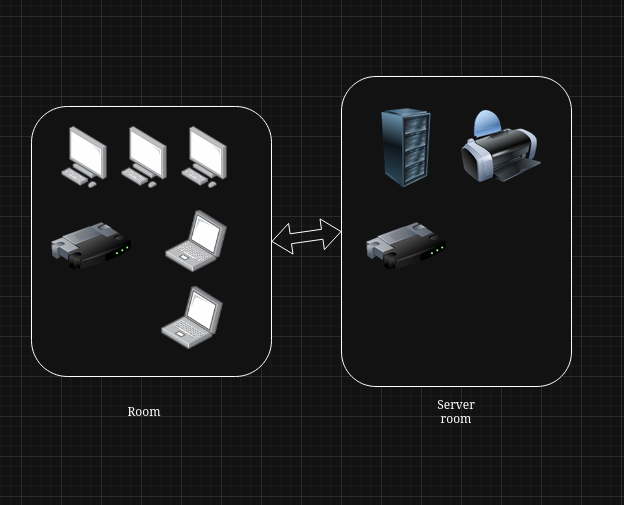
\includegraphics[width=0.75\linewidth]{drawio_deployment.png}
    \caption{Diagram wdrożenia obrazujący architekturę systemu}
    \label{fig:drawio_deployment}
\end{figure}

\clearpage

\section{Visual Paradigm Online - opis działania}
Visual Paradigm Online to narzędzie typu SaaS (Software as a Service), umożliwiające modelowanie UML w przeglądarce. Oferuje:
\begin{itemize}
    \item bogaty zestaw szablonów i symboli UML,
    \item możliwość współpracy zespołowej w czasie rzeczywistym,
    \item integrację z repozytoriami wersji oraz eksport diagramów do różnych formatów.
\end{itemize}
Dzięki dostępności w chmurze projektanci mogą pracować nad modelem z dowolnego miejsca, co znacząco zwiększa elastyczność zespołu projektowego.


\section{Wnioski}
Zastosowanie języka UML w procesie planowania i wdrażania systemów informatycznych pozwala na przejrzyste odwzorowanie zarówno wymagań, jak i architektury rozwiązania. Dzięki różnorodnym typom diagramów możliwe jest spojrzenie na system z różnych perspektyw, od interakcji z użytkownikiem po szczegóły techniczne wdrożenia. 
UML pełni rolę wspólnego języka komunikacji pomiędzy analitykami, programistami i interesariuszami projektu. 
Wnioskiem końcowym jest stwierdzenie, że odpowiednie wykorzystanie UML, wspierane przez dobre narzędzia i praktyki projektowe, znacząco zwiększa efektywność zespołu oraz jakość końcowego produktu informatycznego.

\end{document}